
\documentclass[12pt]{article}
\usepackage{amsmath}
\usepackage{amsfonts}
\usepackage{mathrsfs}
\usepackage{lscape}
\usepackage{listings}
\usepackage{graphicx} % Allows for importing of figures
\usepackage{color} % Allows for fonts to be colored
\usepackage{comment} % Allows for comments to be made
\usepackage{accents} % Allows for accents to be made above and below text
%\usepackage{undertilde} % Allows for under tildes to take place for vectors and tensors
\usepackage[table]{xcolor}
\usepackage{array,ragged2e}
\usepackage{hyperref}
\usepackage{framed} % Allows boxes to encase equations and such
\usepackage{subcaption} % Allows for figures to be side-by-side
\usepackage{float} % Allows for images to not float in the document
\usepackage{booktabs}
%\usepackage[margin=0.75in]{geometry}
\usepackage[final]{pdfpages}
\usepackage{enumitem}
\usepackage[section]{placeins}

%%%%%%%%%%%%%%%%%%%%%%%%%  Function used to generate vectors and tensors %%%%%%%%%
\usepackage{stackengine}
\stackMath
\newcommand\tensor[2][1]{%
	\def\useanchorwidth{T}%
	\ifnum#1>1%
	\stackunder[0pt]{\tensor[\numexpr#1-1\relax]{#2}}{\scriptscriptstyle \sim}%
	\else%
	\stackunder[1pt]{#2}{\scriptscriptstyle \sim}%
	\fi%
}
%%%%%%%%%%%%%%%%%%%

\definecolor{mygrey}{rgb}{0.97,0.98,0.99}
\definecolor{codeblue}{rgb}{.2,0,1}
\definecolor{codered}{rgb}{1,0,0}
\definecolor{codegreen}{rgb}{0.3,0.33,0.12}
\definecolor{codegray}{rgb}{0.5,0.5,0.5}
\definecolor{codepurple}{rgb}{0.55,0.0,0.55}
\definecolor{codecyan}{rgb}{0.0,.4,.4}

\lstdefinestyle{mystyle}{
	backgroundcolor=\color{mygrey},   
	commentstyle=\color{codegreen},
	keywordstyle=\color{codeblue},
	stringstyle=\color{codepurple},
	numberstyle=\tiny\color{codegray},
	basicstyle=\footnotesize,
	breakatwhitespace=false,         
	breaklines=true,                 
	captionpos=b,                    
	keepspaces=true, 
	numbers=left,                    
	numbersep=5pt,                  
	showspaces=false,                
	showstringspaces=false,
	showtabs=false,                  
	tabsize=2
}
\lstset{style=mystyle}

\lstset{language=Matlab,backgroundcolor=\color{mygrey}}
\usepackage{lastpage}
\usepackage{fancyhdr}
\pagestyle{fancy}
%\lhead{\large{Nik Benko, John Callaway, Nick Dorsett, Martin Raming}} 
%\chead{\large{\textbf{ME EN 6960: Lab 1}}}
%\rhead{\today}
\cfoot{[\thepage\ of \pageref{LastPage}]}
\fancyheadoffset{.5cm}
\setlength{\parindent}{0cm}
\usepackage[left=.5in, right=0.50in, top=1.00in,bottom=1.00in]{geometry}
\usepackage{microtype} 
\usepackage{setspace}
\doublespace
%%%%%%%%%%%%%%%%%%%%%%%%%%%%%%%%%%%%%%%%%%%%%%%%%%%%%%%%%%%%%%%%%%%%%%%%%%
% git testing ii

\begin{document}
\title{ Determination of Dynamic Initiation Fracture Toughness Using a Split Hopkinson Pressure Bar  \\ \normalsize{ME EN 6960}}
\author{Nik Benko, John Callaway, Nick Dorsett, Martin Raming}
\maketitle

% John
\begin{abstract} 
In this work, the dynamic initiation fracture toughness of polymethyl methacrylate was quantified using a Split Hopkinson Pressure Bar. A mixed mode fracture toughness locus was created for a strain rate of xx. The crack kinking angle was evaluated as a function of mode mixity. The Maximum Hoop Stress Criterion was compared to experimental results and found to predict higher kinking angles than those found in the experimental data.
\end{abstract}

\section{Introduction} % John

Accurate predictions of dynamic fracture in brittle materials are important for structural design. A major challenge in dynamic material testing is accounting for the inertial effects of a rapidly moving loading apparatus. To overcome this challenge, Kolsky adapted a pressure bar technique originally used by Hopkinson to strike thin material specimens at high speeds \cite{Kolsky}. The long and thin bars of a Split-Hopkinson Pressure Bar (SHPB), combined with a thin material specimen, allow strain measurements from the bars to be analyzed with one dimensional wave analysis. This simplification of three dimensional mechanics down to a single dimension allows for the inertia of the striker bar to be accounted for.
\\ \\
In this report, the dynamic fracture behavior of polymethyl methacrylate (PMMA) will be investigated using a center notch Brazil Disc specimen. The strain rate dependence of Mode I dynamic initiation fracture toughness $K_{1C}$ can be determined by alignment of the Brazil Disc specimen such that the crack is aligned on the axis of the applied dynamic load. Further investigation of mixed mode loading can be completed by rotating the specimen to different angles, creating Mode I and Mode II fracture \cite{Atkinson} \cite{Shetty}. At a given strain rate, the level of mode mixity can be viewed using a mixed mode fracture toughness locus \cite{Nakano}. Finally, the crack kinking angle as a function of mode mixity can by visually confirmed using ImageJ software and compared theoretically to the Maximum Hoop Stress Criterion for crack initiation \cite{Meggiolaro}.  
 
\section{Methods}

\subsection{Experimental Techniques} 

\subsubsection {Split Hopkinson Pressure Bar} % Nick

A Split Hopkinson Pressure Bar (SHPB) is built off of three main parts, the striker bar, the incident bar, and the transmitted bar. A gas gun is used to accelerate the striker bar into the incident bar creating a compression wave down the length of the bar. Upon reaching a sample placed between the incident and transmitted bars, this pulse deforms the sample at a high strain rate, imparting a new compression wave into the transmitted bar. The remainder of the energy is reflected back as a tensile wave. The initial pulse has a wavelength twice the length of the striker bar, necessitating an incident bar length at least four times that of the striker bar.
\\ \\
The biggest working assumption of a SHPB is that the stress wave propagates only along the length of the bar. In order for this to be true, the bar must be made from ma homogenous, isotropic material with a uniform cross section. Additionally, the incident bar material's elastic limit must not be exceeded by the impact of the striker bar. If the length of the bar is at least twenty times greater than its diameter, it can be assumed that the stress is uniform across the cross section. In finite length bars, dispersion must be compensated for as well because different frequencies travel at different speeds. This is done by pulse shaping and post-processing. Pulse shaping is the use of a sacrificial material to reduce the initial slope of the incident pulse to more closely resemble the specimen material response. This reduces the high frequency content of the resulting signal. Post processing equations use known wave velocities to calculate the change in phase angle as the pulse moves down the length of the bar. This then allows the pulse to be reconstructed at any point in time in the form it was at that point. Once the wave has been reconstructed at the instant the specimen began to be strained, the measured voltages are converted into strains. These strains are then used to calculate forces, which in turn are converted into stress if so desired. 

\subsubsection{Dynamic Fracture Mechanics} % Nick

\subsection{Procedure} % Nick
PMMA samples 25 mm in diameter and 3 mm in thickness were prepared with an 8 mm long centered slot in the middle. A razor blade was used to create a small, sharp crack in either side of the slot. Specimens were lightly sanded and had copper contacts glued onto the surface. Thin wires were soldered onto the contacts. Finally, a thin strip of silver conductive paint was drawn across the surface. These prepared samples were loaded into a SHPB with 19.05 mm diameter 7075-T6 aluminum bars. The incident bar was 2.438 m long and the transmitted bar was 1.93 m long. A 1.058 mm thick, 9.525 mm diameter lead pulse shaper was placed between the striker bar and incident bar.
\\ \\
Samples were placed between the incident bar and transmitted bar with the center notch placed at varying angles of inclination. The lead wires hanging off of each sample were attached to the Tektronix DPO 2004B oscilloscope which was being used to record the strain gauge measaurements. This was done as a trigger mechanism, because as the crack propagated it would break the paint and the oscilloscope voltage reading would drop. Strain gauges were placed on each bar approximately in the center, 1.219m from the loading point on the striker bar and 0.965 m from the loading point on the transmitted bar. These were arranged in a full bridge configuration to isolate axial strain. Readings from these strain gauges was taken by the same oscilloscope at 125 MHz with a period of 1 ms. No filtering was used. A gas gun at a pressure of 8 psi was used to accelerate the striker bar.

\subsection{Error and Uncertainties} % Nik/Martin

\section{Results and Discussion} % Nik/Martin

\section{Conclusion} % John
For this report, the evaluation of dynamic properties of polymethyl methacrylate (PMMA) was completed. The dynamic initiation fracture toughness showed a positive correlation with an increase in strain rate. A mixed mode fracture locus was constructed for a strain rate of xx, which showed normalized experimental values below normalized theoretical values. Crack kinking angle was evaluated and compared to predicted kinking angles from the maximum hoop stress criterion. Actual kinking angles were found to be generally lower than predicted values. 

\section{Figures} % Nik/Martin

\begin{figure}[H]
	\centering
	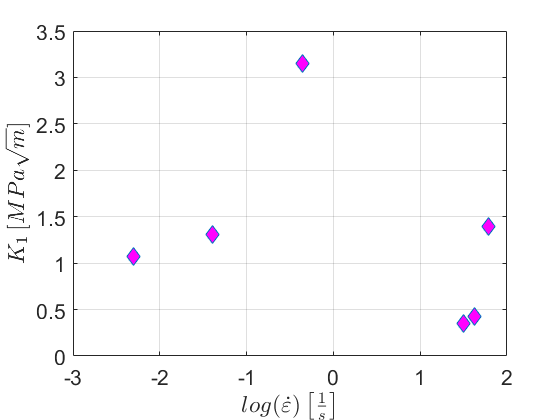
\includegraphics[width=.82\textwidth,scale=1]{Goal1_b.png}
	\caption{}
	\label{fig:Goal1}
\end{figure}

\begin{figure}[H]
	\centering
	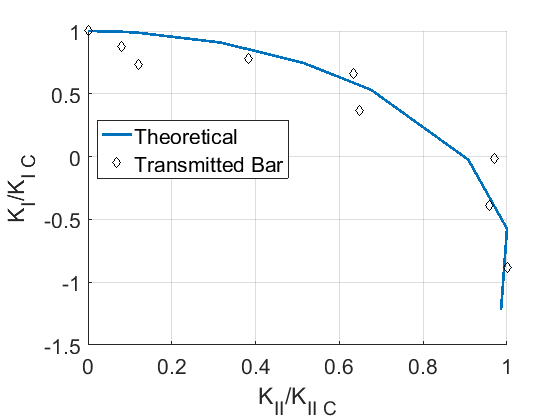
\includegraphics[width=.82\textwidth,scale=1]{Goal2.png}
	\caption{}
	\label{fig:Goal2}
\end{figure}

\begin{figure}[H]
	\centering
	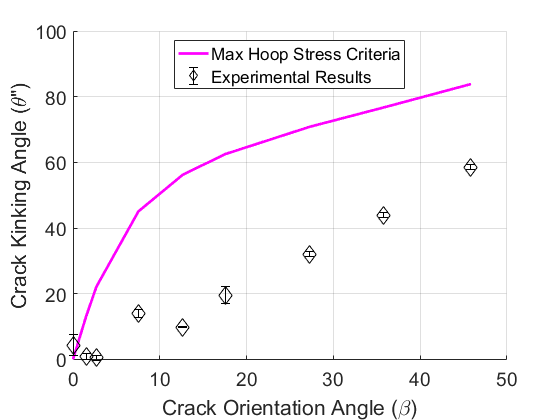
\includegraphics[width=.82\textwidth,scale=1]{Goal3_b.png}
	\caption{}
	\label{fig:Goal3}
\end{figure}


\bibliographystyle{ieeetr}
\bibliography{Lab4Bib}
\end{document}